\documentclass[tikz,border=8pt]{standalone}
\usepackage[T1]{fontenc}
\usepackage{lmodern}
\usepackage{amsmath,amssymb}
\usetikzlibrary{arrows.meta,positioning}
\definecolor{ink}{HTML}{203044}
\definecolor{line}{HTML}{798899}
\definecolor{panel}{HTML}{F4F6F8}
\definecolor{descent}{HTML}{EEF3FA}
\definecolor{physical}{HTML}{EEF5F0}
\definecolor{transport}{HTML}{FCF3EA}
\begin{document}
\pagecolor{white}
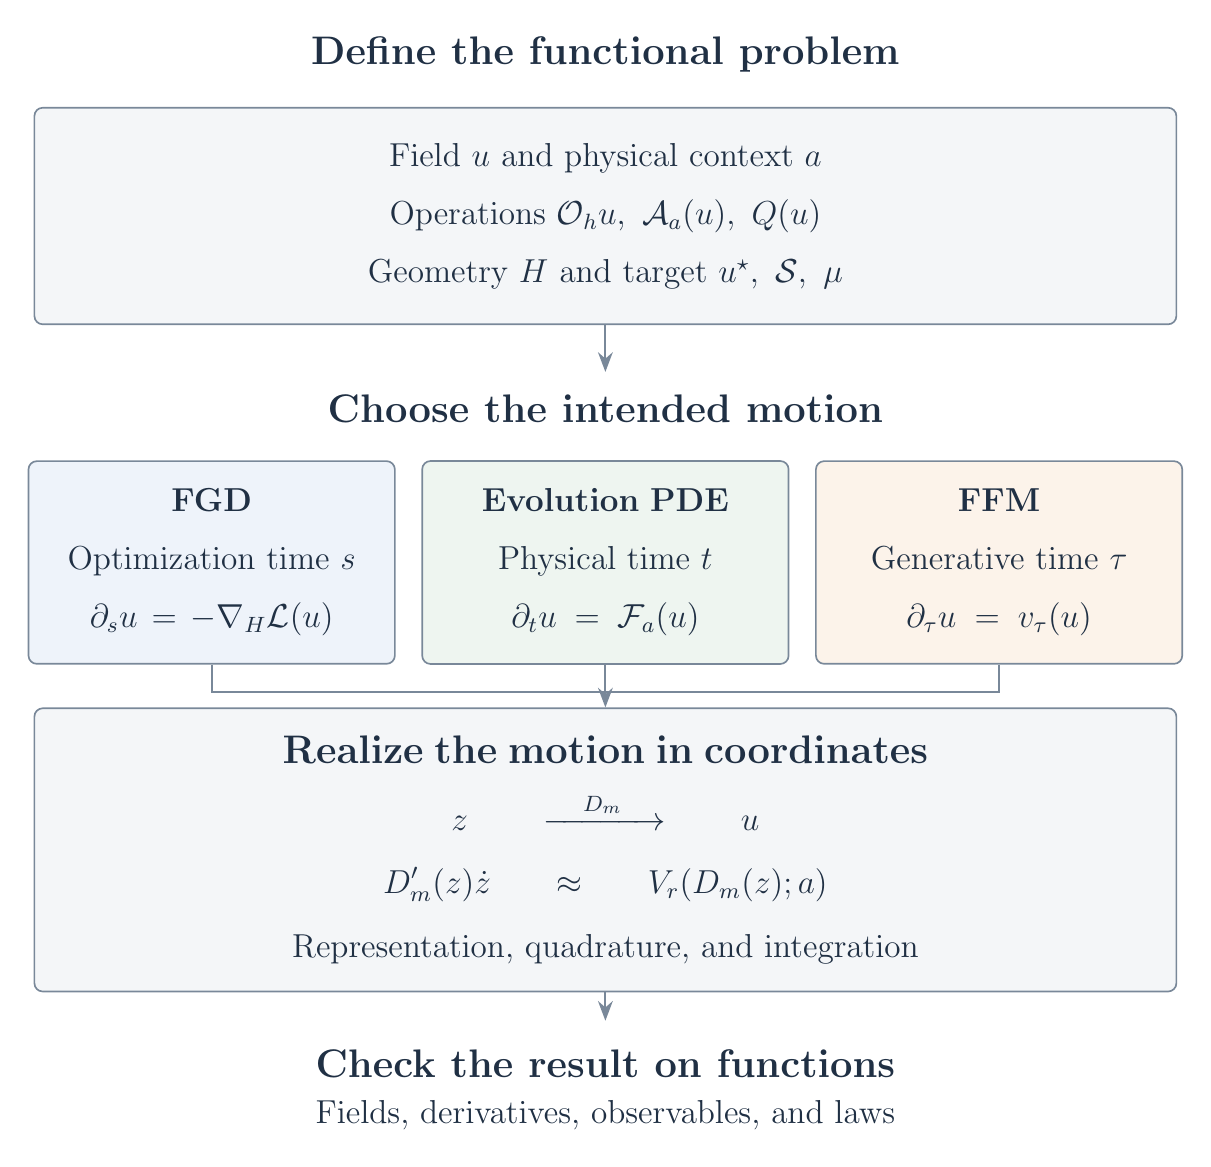
\begin{tikzpicture}[
  text=ink,
  box/.style={draw=line, line width=.6pt, rounded corners=3pt,
    align=center, inner sep=10pt, font=\large},
  heading/.style={font=\Large\bfseries, align=center},
  motion/.style={box, text width=3.95cm, minimum height=2.45cm},
  arrow/.style={-{Stealth[length=2.5mm]}, draw=line, line width=.8pt}
]
  \node[heading] at (0,2.05) {Define the functional problem};
  \node[box, fill=panel, text width=13.8cm, minimum height=2.75cm] (problem) at (0,0) {
    Field \(u\) and physical context \(a\)\\[7pt]
    Operations \(\mathcal O_hu,\ \mathcal A_a(u),\ Q(u)\)\\[7pt]
    Geometry \(H\) and target \(u^\star,\ \mathcal S,\ \mu\)
  };
  \node[heading] at (0,-2.45) {Choose the intended motion};
  \node[motion, fill=descent] (fgd) at (-5,-4.4) {
    \textbf{FGD}\\[7pt]
    Optimization time \(s\)\\[7pt]
    \(\displaystyle \partial_su=-\nabla_H\mathcal L(u)\)
  };
  \node[motion, fill=physical] (pde) at (0,-4.4) {
    \textbf{Evolution PDE}\\[7pt]
    Physical time \(t\)\\[7pt]
    \(\displaystyle \partial_tu=\mathcal F_a(u)\)
  };
  \node[motion, fill=transport] (ffm) at (5,-4.4) {
    \textbf{FFM}\\[7pt]
    Generative time \(\tau\)\\[7pt]
    \(\displaystyle \partial_\tau u=v_\tau(u)\)
  };
  \draw[arrow] (problem.south) -- (0,-1.98);
  \node[box, fill=panel, text width=13.8cm, minimum height=3.15cm] (numerical) at (0,-8.05) {
    {\Large\bfseries Realize the motion in coordinates}\\[10pt]
    \(z \ \xrightarrow{\quad D_m\quad}\ u\)\\[9pt]
    \(\displaystyle D_m'(z)\dot z\ \approx\ V_r(D_m(z);a)\)\\[9pt]
    Representation, quadrature, and integration
  };
  \coordinate (join) at (0,-6.04);
  \draw[draw=line, line width=.8pt] (fgd.south) |- (join);
  \draw[draw=line, line width=.8pt] (ffm.south) |- (join);
  \draw[arrow] (pde.south) -- (numerical.north);
  \node[heading] (check) at (0,-10.77) {Check the result on functions};
  \node[font=\large] at (0,-11.42) {Fields, derivatives, observables, and laws};
  \draw[arrow] (numerical.south) -- (0,-10.22);
\end{tikzpicture}
\end{document}
